\end{multicols*}
\begin{center}
\mysection{Tropes and Species}{adventurer-tropes-species}

\summary {
    Decide if your Adventurer is \mylink{Mortal}{the-inhabitants} or \mylink{Unseelie}{the-inhabitants}.  If you're Mortal, decide which \mybold{Trope} you want to play: \mylink{Sellsword}{trope-sellsword}, \mylink{Knave}{trope-knave}, \mylink{Philosopher}{trope-philosopher}, or \mylink{Mystic}{trope-mystic}. If you're one of the Unseelie, what decide which \mybold{Species} you are: \mylink{\Murk}{species-murk}, \mylink{Pooka}{species-pooka}, \mylink{Night Child}{species-night-child}, or \mylink{Spriggan}{species-spriggan}.

    \myskip

    Grab the appropriate \mylink{Trope Character Sheet}{adventurer-sheet.3} or \mylink{Species Character Sheet}{adventurer-sheet.7} from the appendix, flip to the appropriate section of the book, and follow the creation instructions. Depending on your choices, you'll modify both your sheets (including writing down your \mylink{Flesh}{adventurer-flesh-grit} and \mylink{Grit}{adventurer-flesh-grit}).
}



\end{center}


\begin{multicols*}{2}\raggedcolumns


\mysubsection{Tropes}{adventurer-tropes}

\flavor{And Kib grew weary of the second game, and raised his hand in the Middle of All, making the sign of Kib, and made Men: out of beasts he made them, and Earth was covered with Men. \\~  \Tilde Lord Dunsany}

Mortals are all of the same species (though their appearance varies greatly!); Mortal Adventurers seem to come in four different flavors called \mybold{Tropes}.

\begin{center}
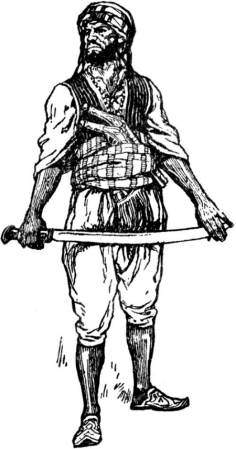
\includegraphics[scale=.6]{adventurer/TropesDetail}
\end{center}


\cbreak

\template{\mybold{\mylink{The Knave}{trope-knave}}}
{You are a thrill-seeker and materialist; a murderer and criminal; a fatalist and hedonist who drinks down life to the last dregs. Thieves, treasure seekers, archaeologists, ruffians, bandits, assassins, etc. belong to this Trope. Knaves are favored with bonuses to their \DEX.}

\template{\mybold{\mylink{The Mystic}{trope-mystic}}}
{You believe in believing; in fate, kismet, and destiny; that we all have a role to play in the Small God's game at the bedside of \TheAuthority. Witches, necromancers, clerics, priests, monks, saints, etc. belong to this Trope. Mystics are favored with bonuses to their \FOC.}


\template{\mybold{\mylink{The Philosopher}{trope-philosopher}}}
{You are a doctor and genius; a dabbler in the madness of the Void; a researcher and alchemist. There is always more to know before \TheEnd, and each question spawns two others. Sorcerers, doctors, wizards, researchers, chemists, healers, etc. belong to this Trope. Philosophers are favored with bonuses to their \INT.}

\template{\mybold{\mylink{The Sellsword}{trope-sellsword}}}
{You are a hammer in a world of nails; a worshiper of violence; a defender and exploiter of the weak. Warriors, fighters, rangers, barbarians, archers, soldiers, etc. belong to this Trope. Sellswords are favored with bonuses to their \VIG.}      

\newpage

\mysubsection{Species}{adventurer-species}

  \flavor{And within the dark circle in which the Freer stood making his curses were no unhallowed things, nor were there strangenesses such as come of night, nor whispers from unknown voices, nor sounds of any music blowing here from no haunts of men; but all was orderly and seemly there and no mysteries troubled the quiet except such as have been justly allowed to man.  And beyond that circle whence so much was beaten back by the bright vehemence of the good man's curses, the will-o'-the-wisps rioted, and many a strangeness that poured in that night from Elfland, and goblins held high holiday. For word was gone forth in Elfland that pleasant folk had now their dwelling in Erl; and many a thing of fable, many a monster of myth, had crept through that border of twilight and had come into Erl to see. And the light and false but friendly will-o'-the-wisps danced in the haunted air and made them welcome.  \Tilde Lord Dunsany }


 The Unseelie are defined by their Species rather than a Trope; though powerful in their own right, they have much less flexibility and choice than the Mortals during Adventurer creation.

\template{\mybold{\mylink{The \Murk}{species-murk}}}  
{"Murks" (as they are more commonly known) are the escaped slaves of the violent and hateful races of the \mylink{Veins of the Earth}{atlas-veins-earth}.  Fallen gods doomed to walk among Mortals, they are forever searching for their way home.  They are often grouped under an epithet \mybold{Rom}, like their cousins the Spriggan. All Murks hail from the Veins of the Earth originally, but they are found throughout the Five Dwarfs near entrances to the Veins.  The horrors they have witnessed (and survived) attunes them to \CLR.}

\template{\mybold{\mylink{The Night Children}{species-night-child}}}
{Night Children are raw Chaos incarnate, taking dozens if not hundreds of different forms.  Creating a Night Child is an entirely random affair, with interesting and powerful results. They are found in every climate, city, and cave throughout the Five Dwarfs. Like their cousins the Pooka, Night Children are thought to somehow be blessed by Chaos, and exhibit a degree of "luck" that attunes them to \TAL.}

\template{\mybold{\mylink{The Pooka}{species-pooka}}}
{Drug-crazed and thought to be half-lapin, Pooka are widely sought by adventuring Bands for their uncanny good fortune. Pooka are most comfortable around others (Mortal or otherwise), and thus hail from any \mylink{Settlement}{civilization-settlements}.  When they aren't adventuring, they commonly find work as sailors, jesters, scouts, and tavern keepers - but rarely gamblers, since no one will play with them.  Their natural charisma and charm attunes them to \PRE.}



\template{\mybold{\mylink{The Spriggan}{species-spriggan}}}
{Ex-vassals of the King of Elfland, wandering the Mortal lands trying to find the bright line of Elfland again.  They are able to summon and control \mylink{The Forgotten}{remembrance} - animals, demons, and forgotten gods - and forge legendary \mylink{magical blades}{wonder-sword-magic}.  Like the \Murk they are often called \mybold{Rom}.  All Spriggan hail from Elfland originally, though they can often be found near towns and cities bordering the \mylink{the Weald}{atlas-elfland-weald}. Spriggan have "the Sight", a supernaturally attuned \AWA of their surroundings.}
    

